\chapter{Propuesta de alto nivel}

En este proyecto se tiene como objetivo el diseño y la implementación de un sistema ciberfísico basado en un robot móvil omnidireccional, el cual será utilizado como plataforma para estudiar y modelar el comportamiento de un sistema compuesto por un robot que sigue trayectorias predefinidas calculadas mediante algoritmos de planificación.

La propuesta, por un lado, incluye el desarrollo de un sistema de locomoción omnidireccional compuesto por cuatro ruedas, lo que permitirá al robot moverse en cualquier dirección. Por el otro, se integra una interfaz de usuario para  control y supervisión del comportamiento de los robots.

Para abordar los desafíos del control y la coordinación en entornos compartidos, implica que se tenga un enfoque que permita representar de manera estructurada las restricciones del entorno, garantizar la exclusividad en regiones críticas y asegurar una gestión ordenada de los recursos. Esta estrategia facilita la sincronización entre robots previene situaciones de conflicto.

Al mismo tiempo, implícitamente vemos que es necesario un mecanismo de localización espacial, esto se puede lograr mediante la fusión de datos provenientes de múltiples sensores, lo cual permite mantener información confiable y actualizada sobre el estado del sistema. En conjunto, estas capacidades contribuyen a una navegación autónoma más segura, eficiente y robusta. \cite{papermico} \cite{negenborn2003robot}

\begin{figure}[H]
    \centering
    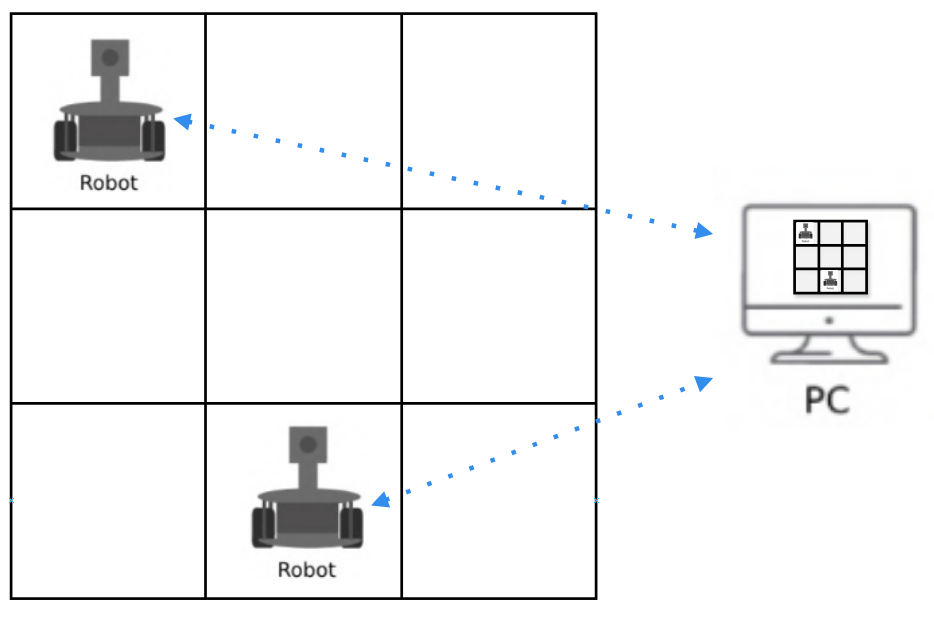
\includegraphics[width=0.65\linewidth]{mt_alto-nivel.png}
    \caption{Propuesta de alto nivel}
    \label{fig:propaltonivel}
\end{figure}

